
\chapter{Introducción específica}  
 
 
Este capítulo explora los requisitos fundamentales para el desarrollo de un sistema de chatbot, que abarcan aspectos funcionales, de documentación, pruebas, interfaz y rendimiento. Además, revisa los diferentes tipos de chatbots y modelos de inteligencia artificial, con énfasis en sus características y aplicaciones en el procesamiento de lenguaje natural.


\section{Requerimientos}

\begin{enumerate}
    \item Requerimientos funcionales:
        \begin{enumerate}
            \item El sistema debe ser capaz de procesar y comprender mensajes de texto entrantes.
            \item El chatbot debe poder proporcionar respuestas relevantes y precisas a las consultas de los usuarios.
            \item Los usuarios deben tener la posibilidad de interactuar con el chatbot a través de una interfaz de usuario.
            \item Se requiere una interfaz de usuario que facilite el proceso de reentrenamiento del chatbot mediante el uso de los historiales de conversación.
        \end{enumerate}
    \item Requerimientos de documentación:
        \begin{enumerate}
            \item Documentar detalladamente las tecnologías utilizadas y sus principales características, así como las particularidades de diseño de cada una.
            \item El sistema no almacenará datos personales de los usuarios, sino que se limitará a responder preguntas frecuentes. En caso de requerirse almacenamiento de datos, se utilizará una plataforma con medidas de seguridad integradas, como autenticación mediante logins con Google.
            \item Entregar una memoria técnica que contenga información detallada sobre la implementación del sistema, que incluya aspectos técnicos, arquitectura y decisiones de diseño.
            \item Proporcionar un registro de avance que documente los hitos alcanzados durante el desarrollo del proyecto, que contemple fechas de cumplimiento y descripciones de las tareas realizadas.
         \end{enumerate}
		 
	\newpage % agrego un salto de página 
    \item Requerimientos de Testing:
        \begin{enumerate}
            \item Se llevarán a cabo pruebas en diferentes escenarios y con diferentes tipos de contexto de datos, para garantizar la fiabilidad y precisión del chatbot.
         \end{enumerate}
    \item Requerimientos de la Interfaz:
        \begin{enumerate}
            \item Se requiere una interfaz interactiva, que permita hacer preguntas y obtener respuestas en tiempo real dentro del mismo entorno de interacción.
        \end{enumerate}
    \item Requerimientos de Rendimiento:
        \begin{enumerate} 
            \item Se establece un límite máximo de tiempo de respuesta de 1 minuto, para asegurar una experiencia satisfactoria para el usuario.
        \end{enumerate}
  \end{enumerate}


  \section{Modelos de inteligencia artificial para PLN}
  El procesamiento de lenguaje natural (PLN) ha avanzado significativamente gracias al desarrollo de diversas técnicas de inteligencia artificial. Estas se pueden clasificar en varias categorías, cada una con su propio enfoque y aplicación.
     
  \textbf{Modelos basados en reglas:} estos modelos utilizan gramáticas y diccionarios para analizar el lenguaje. Aunque son efectivos en tareas específicas, su rigidez y la necesidad de una extensa programación manual limitan su aplicabilidad en contextos más amplios.
  
  \textbf{Modelos estadísticos:} a medida que los datos comenzaron a acumularse, los modelos estadísticos, como los n-gramas, se convirtieron en populares. Estos modelos predicen la probabilidad de una palabra en función de las palabras anteriores. Sin embargo, su dependencia de datos limitados puede resultar en un contexto insuficiente, lo que afecta la calidad de las predicciones.
  
  \textbf{Modelos de aprendizaje profundo:} con el auge del aprendizaje profundo, arquitecturas como RNN (Redes Neuronales Recurrentes), LSTM (Memoria a Largo Plazo) y transformers han revolucionado el PLN. Estos modelos pueden captar patrones complejos en grandes volúmenes de datos, lo que les permite realizar tareas como la traducción automática y la generación de texto de manera más efectiva.
  

  \subsection{Modelos de Lenguaje modernos}

  Modelos como BERT (Bidirectional Encoder Representations from Transformers) y GPT (Generative Pre-trained Transformer) han transformado el campo del procesamiento de lenguaje natural (PLN), al ofrecer enfoques innovadores para comprender y generar texto.
  
  \begin{itemize}
	  \item \textbf{GPT}: este modelo utiliza técnicas de aprendizaje profundo para generar texto coherente y contextualmente relevante. Su capacidad para crear respuestas naturales ha revolucionado la interacción de los chatbots con los usuarios, lo que permite conversaciones más fluidas y precisas.
  
	  \item \textbf{BERT}: a diferencia de otros modelos, BERT se centra en el análisis bidireccional del texto, lo que le permite entender el contexto de manera más profunda. Esta característica mejora la identificación de intenciones y la respuesta a preguntas complejas, lo que ayuda a crear chatbots más competentes en diálogos matizados.
  \end{itemize}
  

  \section{Modelos de chatbots: RAG vs Fine-Tuning}
  
  Los chatbots se pueden clasificar según sus arquitecturas y métodos de entrenamiento. Entre las más destacadas se encuentran Retrieval Augmented Generation (RAG) y fine-tuning. Ambas arquitecturas ofrecen ventajas complementarias, lo que las convierten en opciones populares en el desarrollo de chatbots efectivos \cite{greyling2023}.



  
  \subsection{Retrieval Augmented Generation (RAG)}
  
  RAG combina la generación de lenguaje natural con la recuperación de información, enfocándose principalmente en una \textit{knowledge base}\footnote{knowledge base [base de conocimiento].}. Cuando un usuario formula una pregunta, RAG utiliza \textit{embeddings}\footnote{embeddings [representaciones vectoriales].} para identificar y recuperar las partes del \textit{relevant knowledge}\footnote{relevant knowledge [conocimiento relevante].} que son pertinentes a esa pregunta.
  Este conocimiento relevante se inyecta en el \textit{prompt}\footnote{prompt [entrada o solicitud al modelo de lenguaje].} enviado al modelo de lenguaje (LLM). El \textit{prompt} incluye tanto la pregunta como el contexto relacionado, lo que permite a la LLM generar respuestas más precisas y contextualizadas. La incorporación de datos externos en este proceso enriquece el conocimiento del modelo en tiempo real y disminuye las posibilidades de \textit{hallucinations}\footnote{hallucinations [alucinaciones].}—respuestas que, aunque parecen plausibles, son incorrectas.
  Además, RAG utiliza bases de datos vectoriales y la búsqueda semántica para recuperar información relevante, lo que mejora la precisión y relevancia de las respuestas del chatbot. Este enfoque es especialmente útil en situaciones donde se requiere información actualizada o especializada, como en consultas de productos o en el soporte técnico.

%  \vspace{1cm}
 \begin{figure}[htbp] 
	\centering
	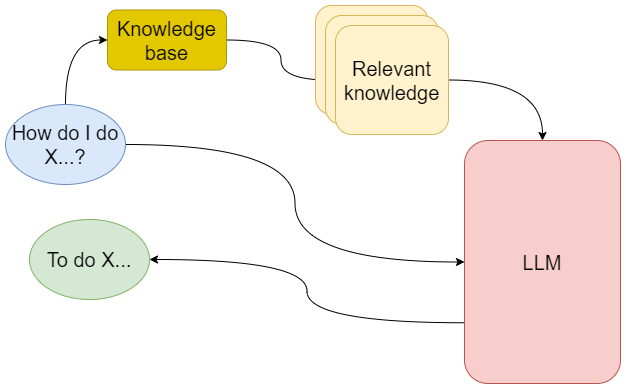
\includegraphics[width=.75\textwidth]{./Figures/RAG.png}
	\caption{Diagrama de flujo de una consulta en un chatbot con arquitectura RAG.}
	\label{fig:arquitectura_rag}
\end{figure}
% \vspace{1cm}

  \newpage
  
  \subsection{Fine-Tuning}
  El fine-tuning implica ajustar un modelo de lenguaje preentrenado en un conjunto de datos específico para mejorar su comportamiento en contextos particulares. Este proceso optimiza la efectividad del modelo en aplicaciones industriales específicas, como en medicina, derecho o ingeniería. Sin embargo, una desventaja del fine-tuning es que el modelo resultante puede quedar congelado en un estado particular, lo que limita su adaptabilidad a nuevos contextos sin un nuevo ciclo de entrenamiento.
  Aunque el fine-tuning proporciona respuestas más precisas en contextos específicos, también puede carecer de la flexibilidad de RAG, que permite incorporar datos contextuales en tiempo real.
   
  \newpage
\subsection{Ventajas y desventajas de los modelos RAG y Fine-Tuning}
  
  Esta subsección presenta una comparación entre ambos modelos, que muestra sus ventajas y desventajas.
  \begin{table}[ht]
    \centering
    \caption{Ventajas y desventajas de los modelos RAG y Fine-Tuning.}
    \begin{tabular}{|c|p{0.35\linewidth}|p{0.35\linewidth}|}
        \hline
        % \textbf{Modelo} & \textbf{Ventaja} & \textbf{Desventaja} \\
        \multicolumn{1}{|c|}{\textbf{Modelo}} & \multicolumn{1}{c|}{\textbf{Ventaja}} & \multicolumn{1}{c|}{\textbf{Desventaja}} \\ 
        \hline
        RAG & 
        \begin{raggedright}
        \begin{itemize}
            \item Permite incorporar información contextual actualizada en tiempo real.
            \item Reduce la probabilidad de alucinaciones al usar datos relevantes.
            \item Mejora la precisión y relevancia de las respuestas del chatbot.
        \end{itemize} 
        \end{raggedright} & 
        \begin{raggedright}
        \begin{itemize}
            \item Requiere una infraestructura adecuada para la recuperación de información.
            \item Dependencia de la calidad y disponibilidad de la base de datos.
            \item Puede ser más complejo de implementar y mantener.
        \end{itemize} 
        \end{raggedright} \\
        \hline
        Fine-Tuning & 
        \begin{raggedright}
        \begin{itemize}
            \item Mejora la calidad de las respuestas al adaptar el modelo a un dominio específico.
            \item Proporciona un rendimiento más consistente en contextos bien definidos.
            \item Permite la optimización de la latencia al trabajar con un modelo entrenado.
        \end{itemize} 
        \end{raggedright} & 
        \begin{raggedright}
        \begin{itemize}
            \item El modelo se congela en el tiempo y no se adapta a cambios contextuales.
            \item Requiere un conjunto de datos específico para el entrenamiento, lo que puede ser costoso.
            \item Menor flexibilidad para abordar consultas inesperadas o no entrenadas.
        \end{itemize} 
        \end{raggedright} \\
        \hline
    \end{tabular}
    \label{tab:rag_vs_finetuning}
\end{table}

 